\section[Differential branching fraction measurements of the decay \btokpipimumu]{
  Differential branching fraction measurements of the decay \tmath{\btokpipimumu}
}
%Binning scheme in
      %decays~\cite{LHCb-PAPER-2013-017,LHCb-PAPER-2013-037,LHCb-PAPER-2013-019}.

Given the statistics available for this channel, the differential branching fraction,
$\dBF(\btokpipimumu)/\dqsq$ was calculated in bins of \qsq.
The differential branching fraction for a bin of width $\Delta\qsq$ is
%\begin{equation}
  %\frac{d}{\dqsq}\BF\left(\btokpipimumu\right)
  %=
  %\frac{\num{sig}}{\num{norm}} \cdot
  %\frac{\eff{norm}}{\eff{sig}} \cdot
  %\frac{\BF_\mathrm{tot}\left(\btopsitwosk\right)}{\Delta\qsq}
%\end{equation}
\begin{equation}
  \frac{d}{\dqsq}\BF\big(\btokpipimumu\big)
  =
  \frac{N(\kpipi\mumu)}{N\big(\psitwos\Kp\big)} \cdot
  \frac{\varepsilon\big(\psitwos\Kp\big)}{\varepsilon\big(\kpipi\mumu\big)} \cdot
  \frac{\BF_\mathrm{tot}\big(\btopsitwosk\big)}{\Delta\qsq}
  \label{eq:kpipi:diffbf}
\end{equation}
where,
\begin{equation}
  \BF_\mathrm{tot}\big(\btopsitwosk\big)
  =
  \BF\big(\btopsitwosk\big) \cdot
  \BF\big(\psitwostojpsipipi\big) \cdot
  \BF\big(\jpsitomumu\big),
\end{equation}
\num{sig} is the yield of the signal decay \btokpipimumu in the given \qsq bin and \num{norm}
is the yield of the normalization channel.
Total efficiencies for reconstruction and selection are denoted by \eff{sig} and \eff{norm} for the
signal and normalization channels respectively.

The normalization channel was chosen to be \btopsitwosk, where \psitwostojpsipipi and \jpsitomumu,
which has a total branching fraction of $(1.264 \pm 0.0052)\e{-5}$~\cite{PDG2012}.
This was chosen for the normalization channel over the decay \btojpsikpipi because it has a relative
uncertainty of $4\,\%$ rather than $16\,\%$ for $\BF(\btojpsikpipi) = (8.1\pm1.3)\e{-4}$.

the yield  of the normalization channel is extracted from an unbinned extended maximum likelihood
fit to the invariant mass distribution of \btopsitwosk candidates.
The function used to fit the data constitiutes a signal and background component.
Signal candidates are modelled using the sum of two Gaussian functions, each having a power-law
tail at low-mass.
The paramters of the tail shared between the Gaussians, and all parameters are taken from a fit to
the high statistics mode of the cross-check channel \btojpsikpipi.
The background function is made of en exponential --- to model combinatorial background --- and a
Gaussian --- to model partially reconstructed candidates --- at low mass.
The same function is used to fit $m(\jpsi\kpipi)$ the control channel.
These fits are shown in \Fig{fig:kpipi:norm} and they yield
$N(\psitwos\Kp)=5128\pm67$ and $N(\jpsi\kpipi)=59\,335\pm343$.

\begin{figure}
  \begin{center}
    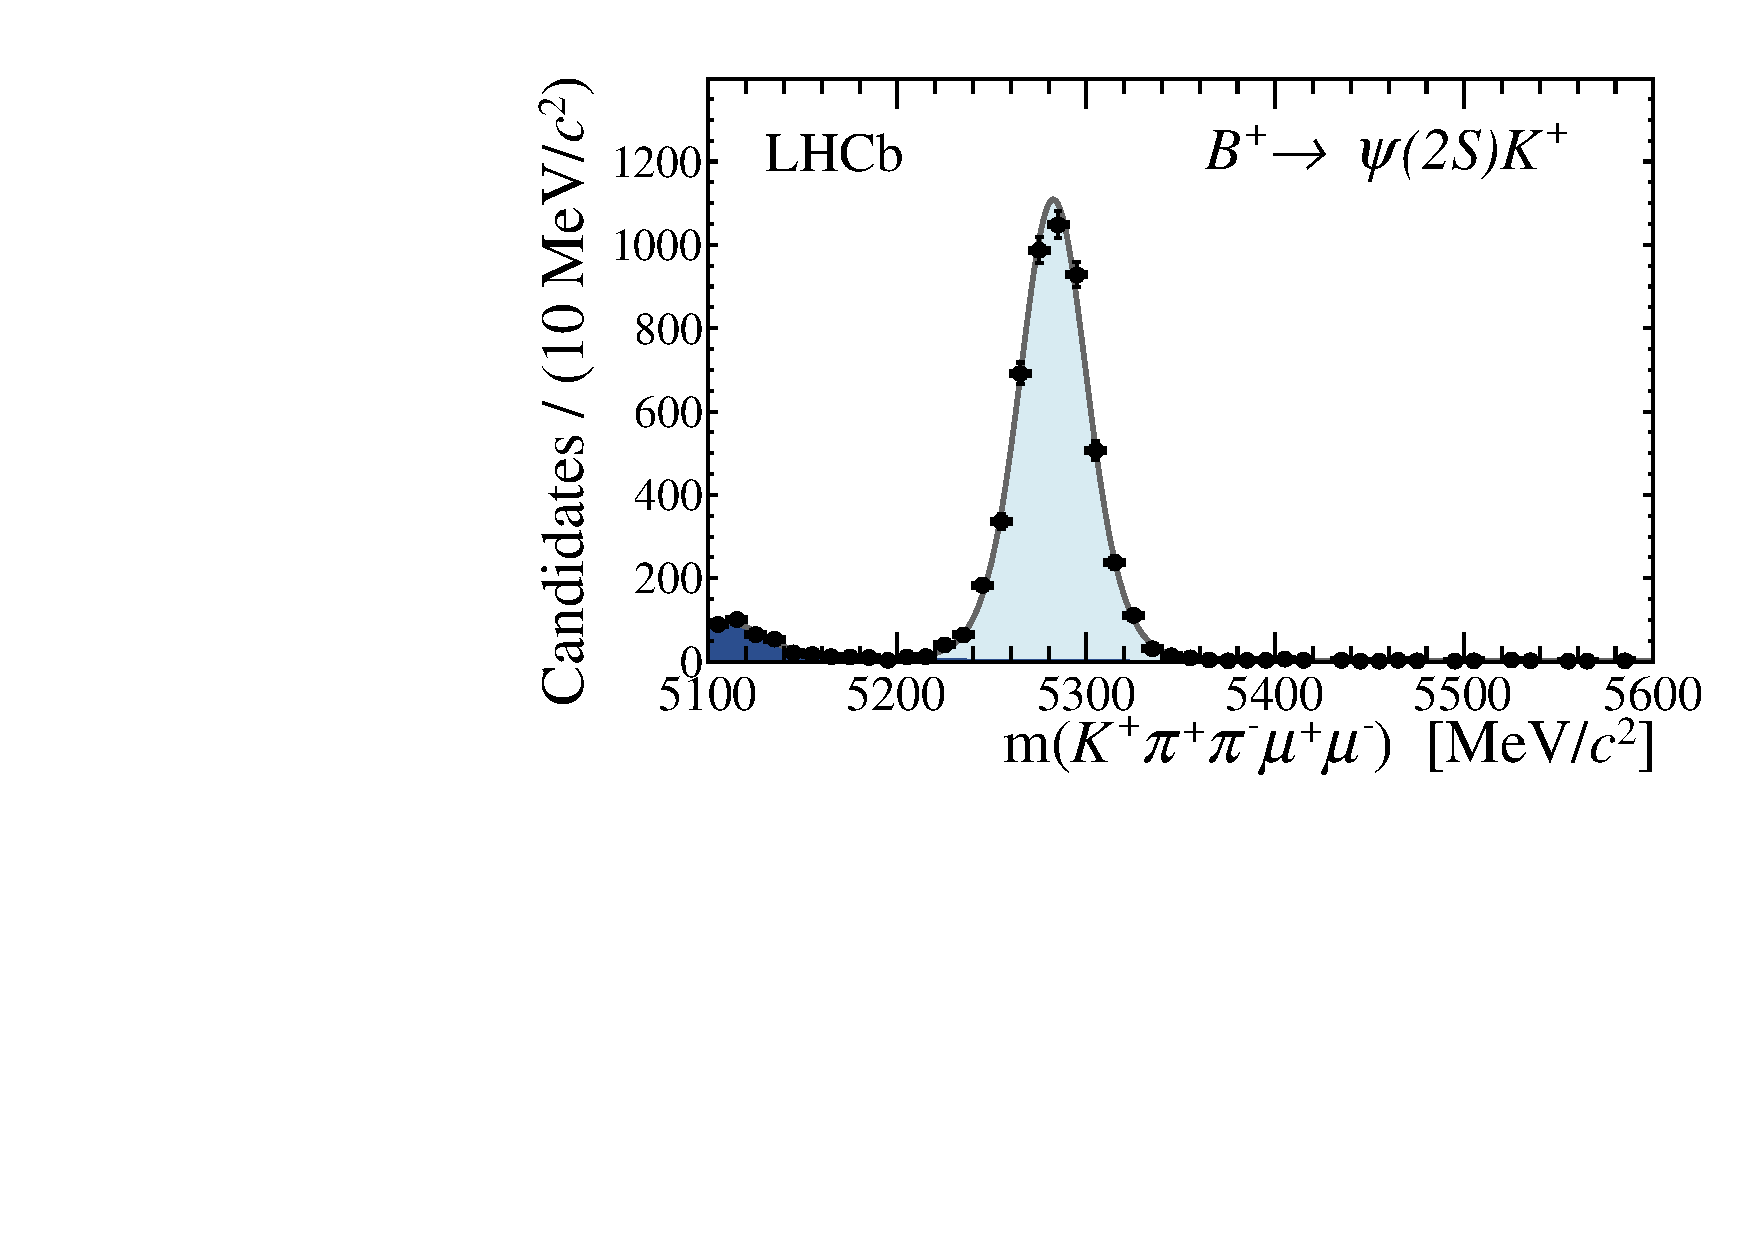
\includegraphics[width=0.48\textwidth]{b2psi2sk}
    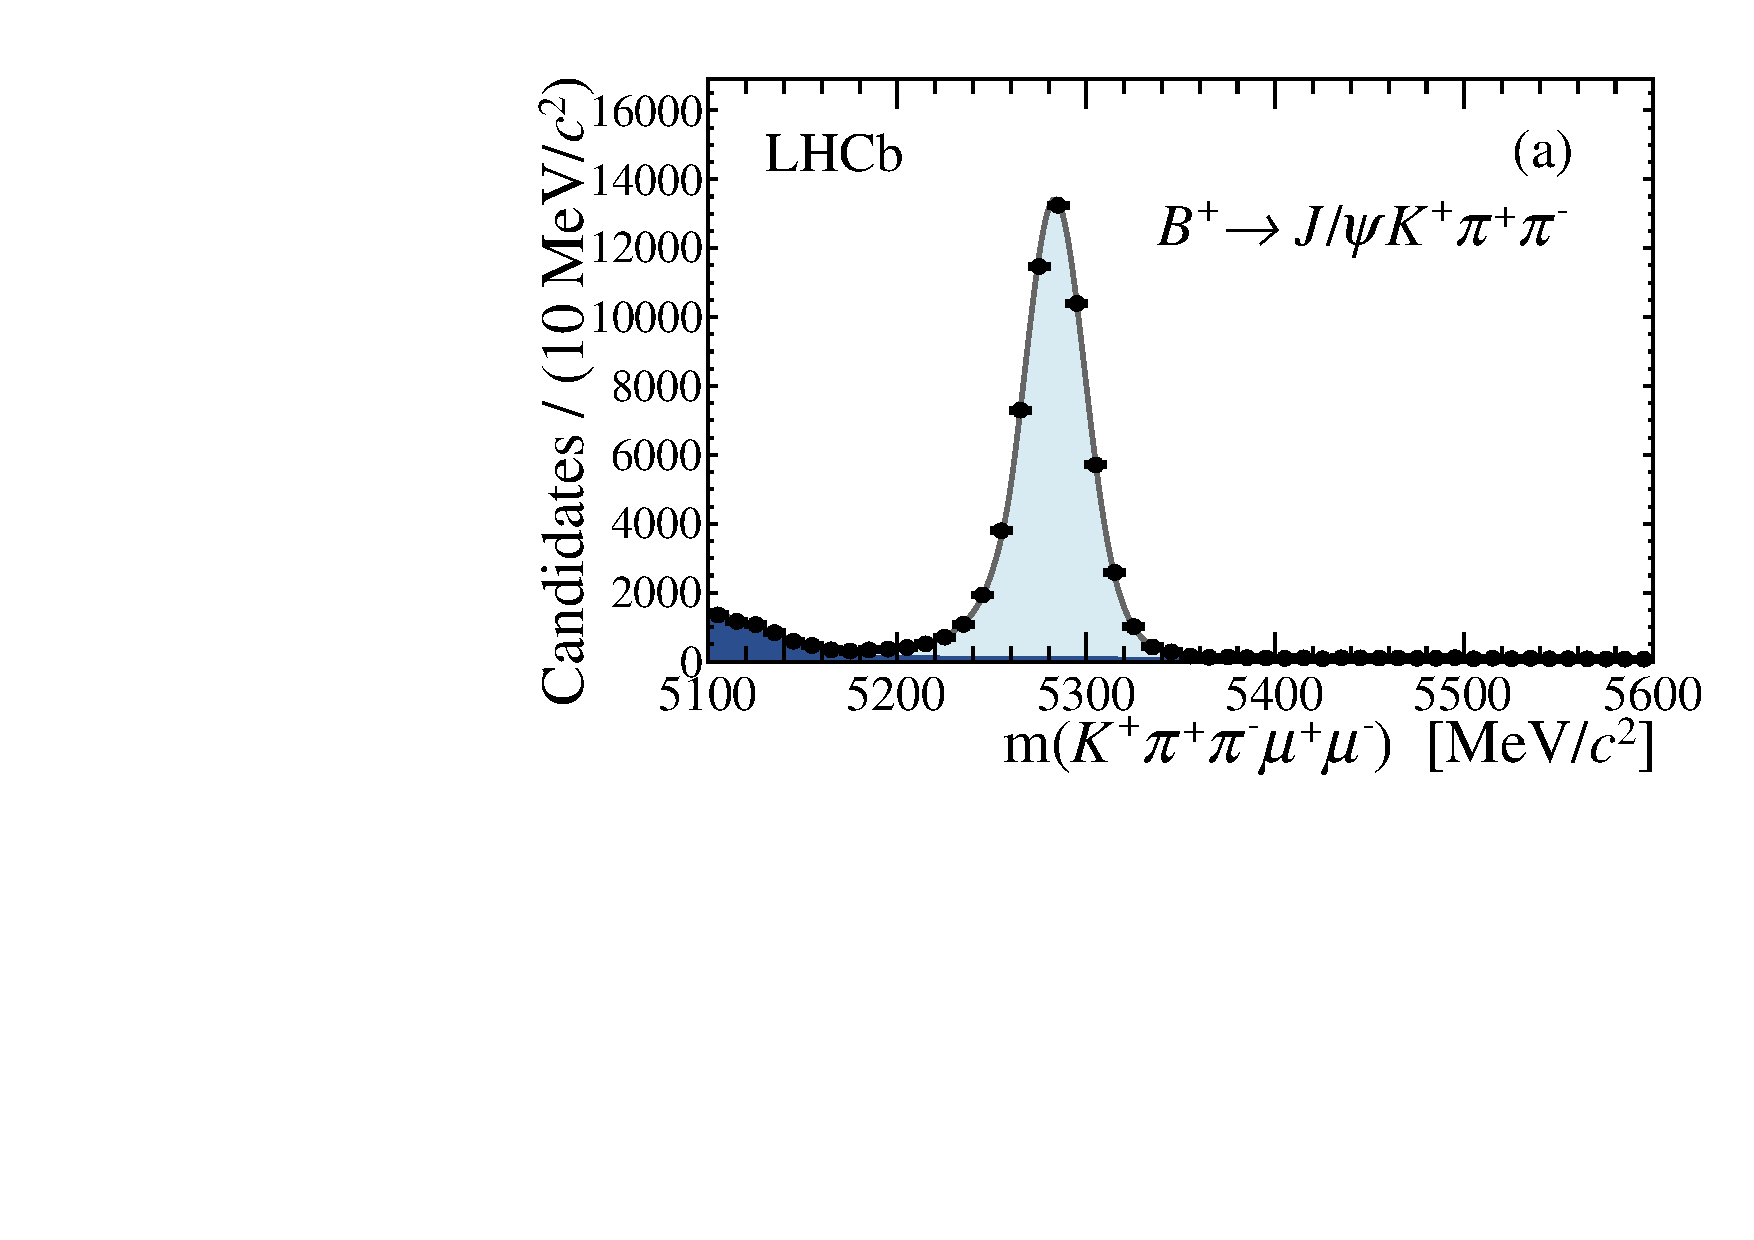
\includegraphics[width=0.48\textwidth]{b2kpipijpsi}
    \caption{\small
      Distributions of the invariant mass of the
      (a) cross-check channel \btojpsikpipi and
      (b) normalization mode \btopsitwosk.
      Projections from the fit are overlayed, where the light blue is the yield of the indicated
      decay, and the dark blue is the background component.
    }
    \label{fig:kpipi:norm}
  \end{center}
\end{figure}

%Just as in the signal fits, the normalization background is an exponential, but accounts to the
%partially reconstructed background at low mass with a Gaussian.
%Signal function is also a \bam{Something here}.
%The fitted invariant mass distribution for \btopsitwosk candidates is shown in
%\Fig{fig:kpipi:norm}, which yields $N(\psitwos\Kp)=5128\pm67$ normalization candidates.


Yields of the signal decay in regions of \qsq were extracted from fits using a distribution that
was fixed to as large an extent as possible.
The lower limit of the fit was taken to be $5150\mev$, because partially recontructed background
is a problem below that.
The combinatorial backgorund shape is an exponential distribution, where the exponent and yield was
allowed to float in the fit; however, in the regions where charmonium vetoes are effective, the
steps in the background are fixed using sideband data.
The signal function was a \bam{Cant remember, double or single Crystal Ball}, where all the shape
parameters were fixed in a fit to the cross-check decay \btojpsikpipi.
Figure~\ref{fig:kpipi:q2fits} shows the invariant mass distribution for all \btokpipimumu
candidates for the whole \qsq region and for each bin.
The total yield of \btokpipimumu candidates is $N(\kpipi\mumu)=367\,^{+24}_{-23}$.

\begin{figure}
  \begin{center}
    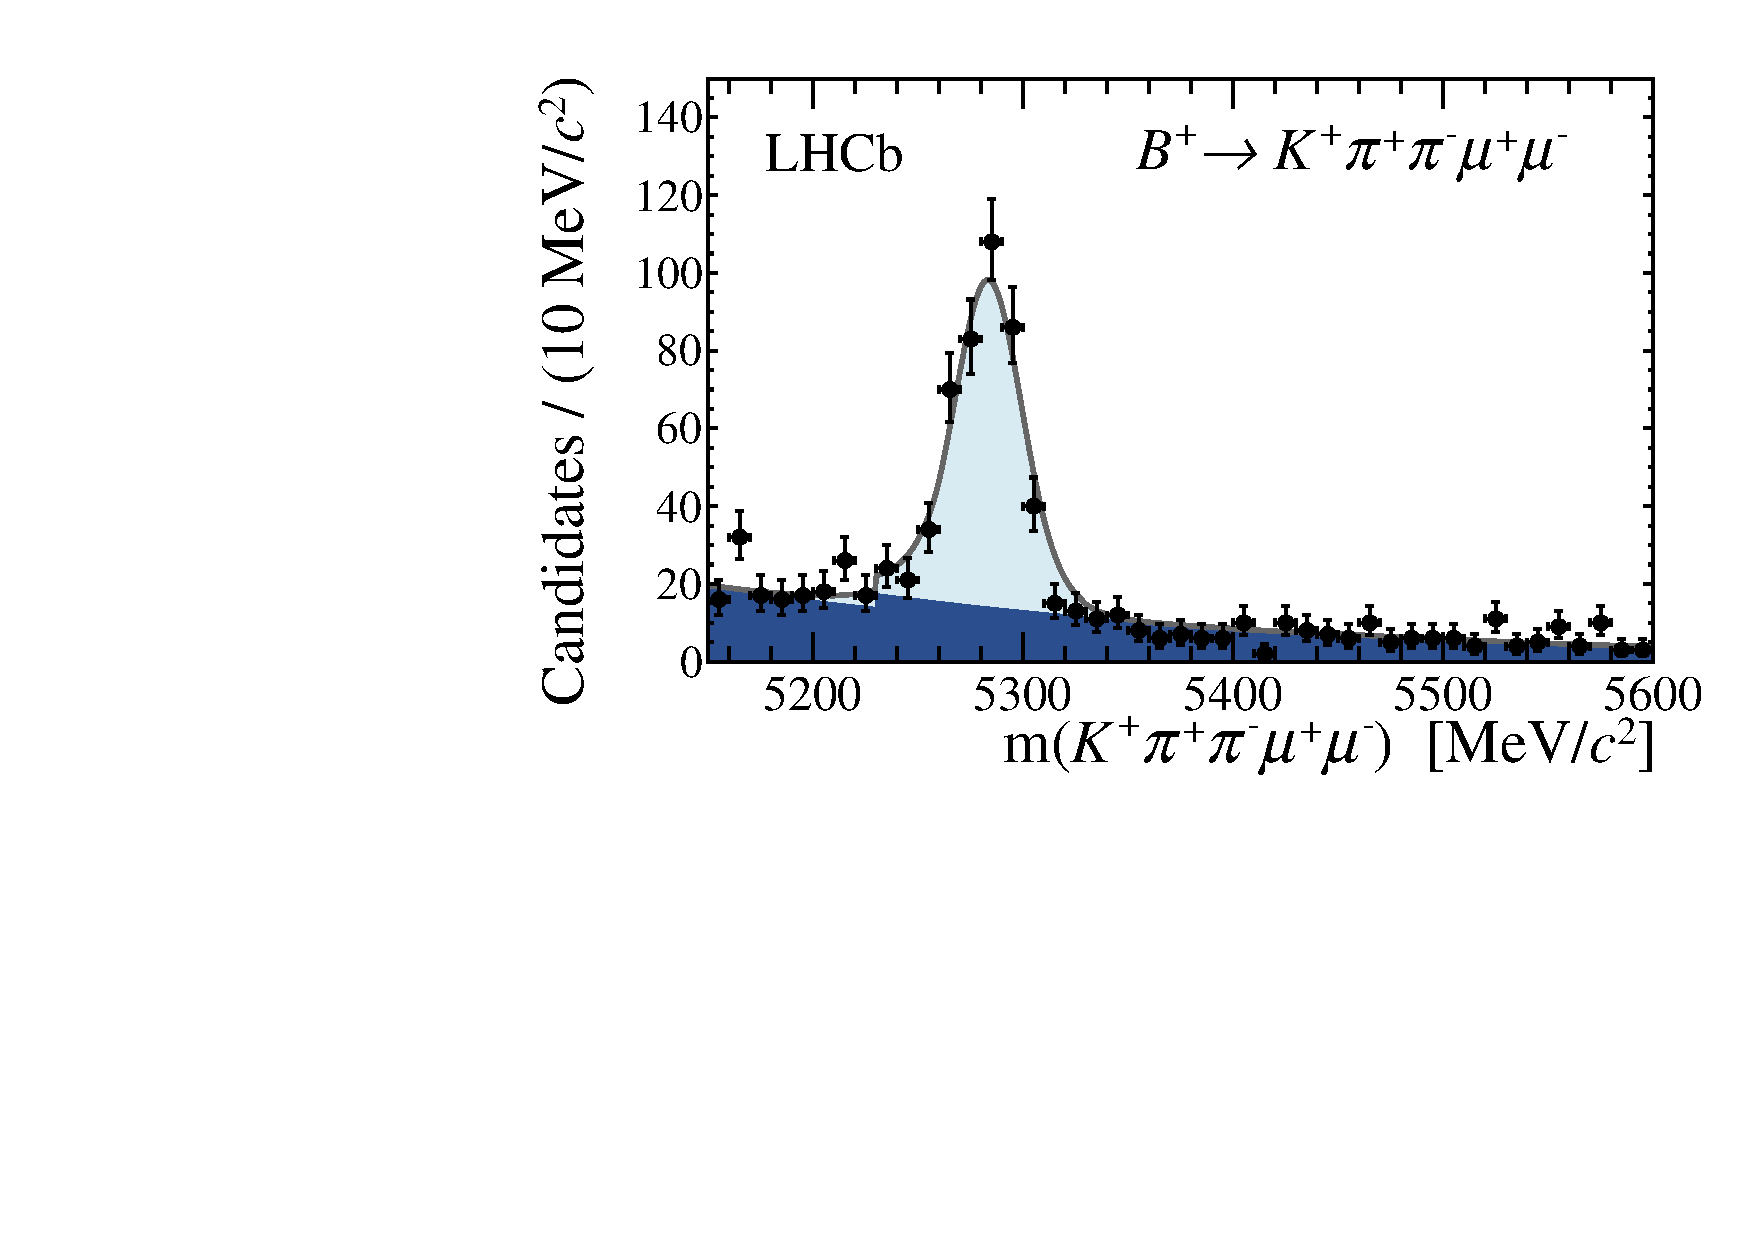
\includegraphics[width=0.48\textwidth]{b2kpipimumu}
    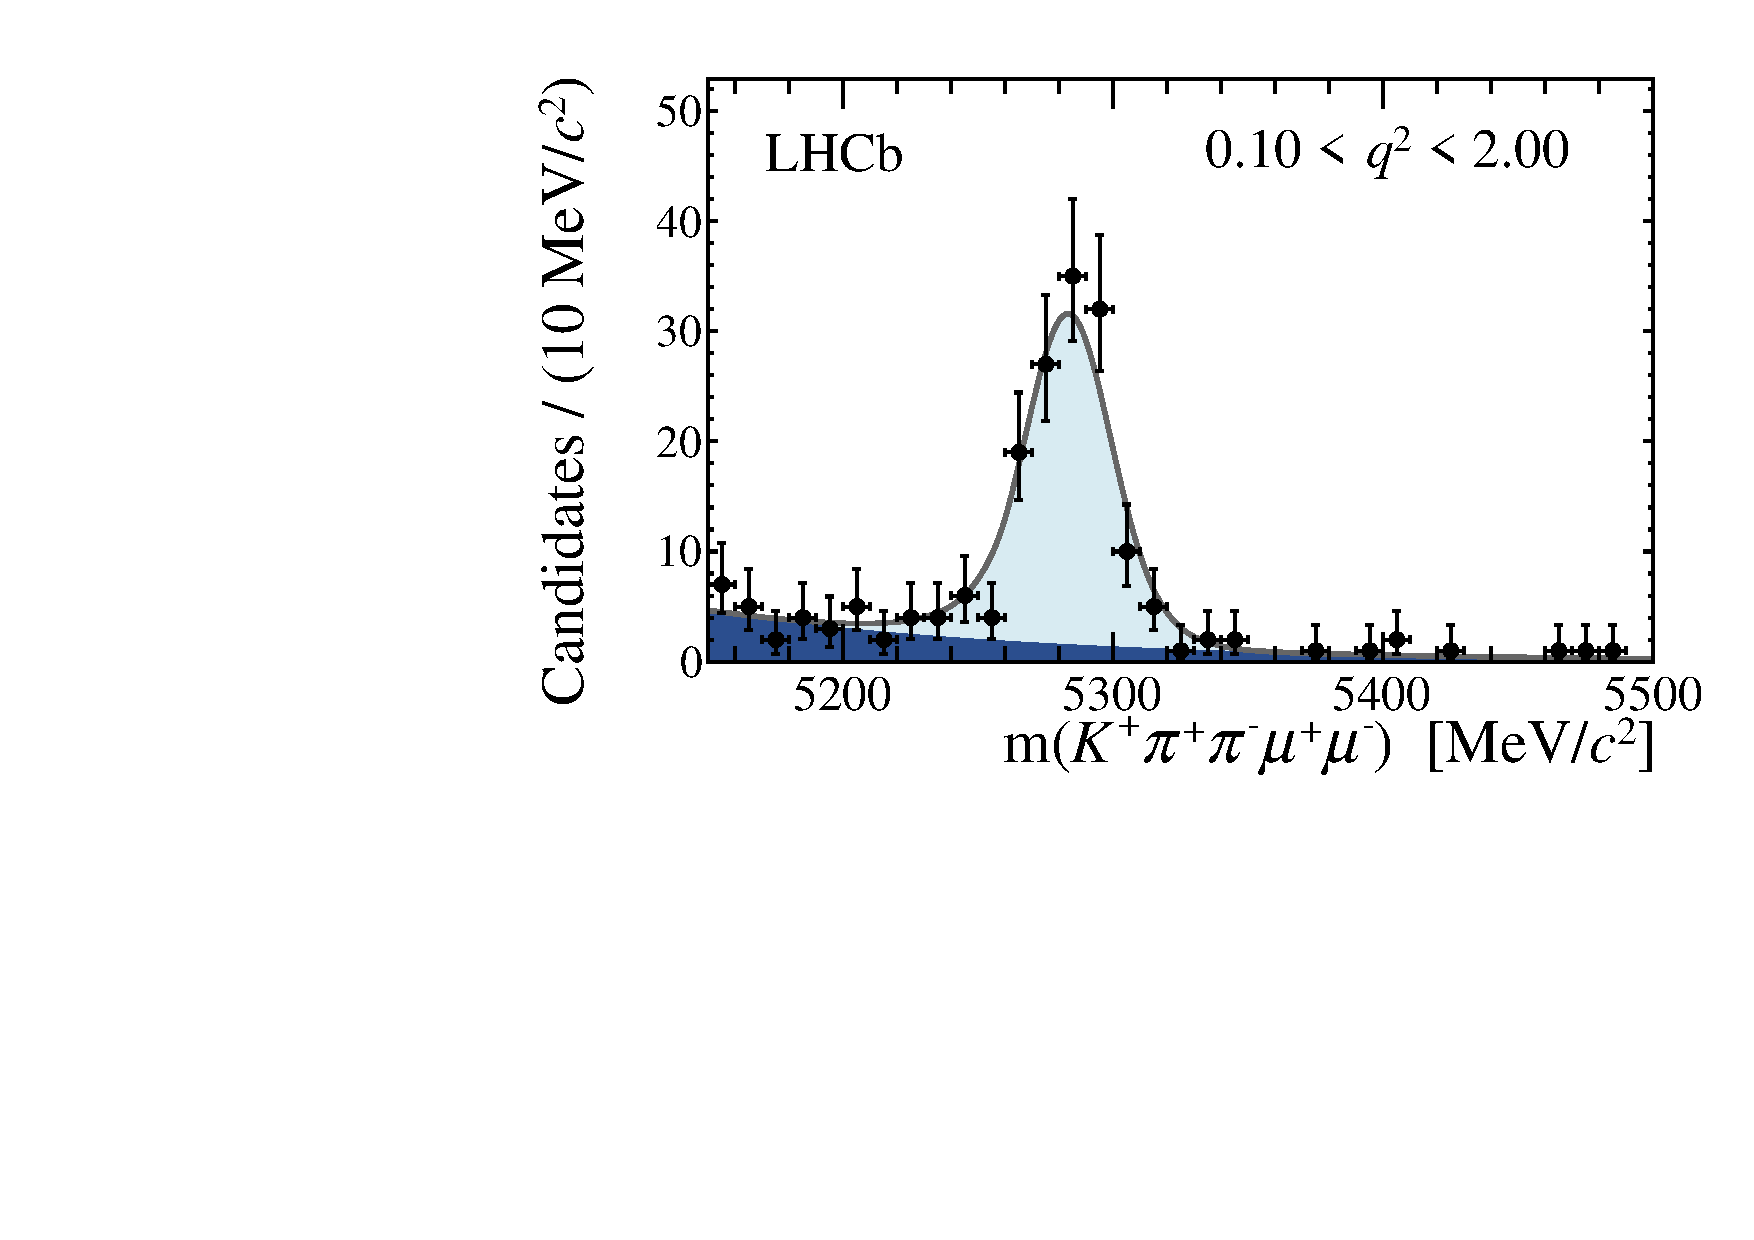
\includegraphics[width=0.48\textwidth]{kpipimumu_q2_r2}
    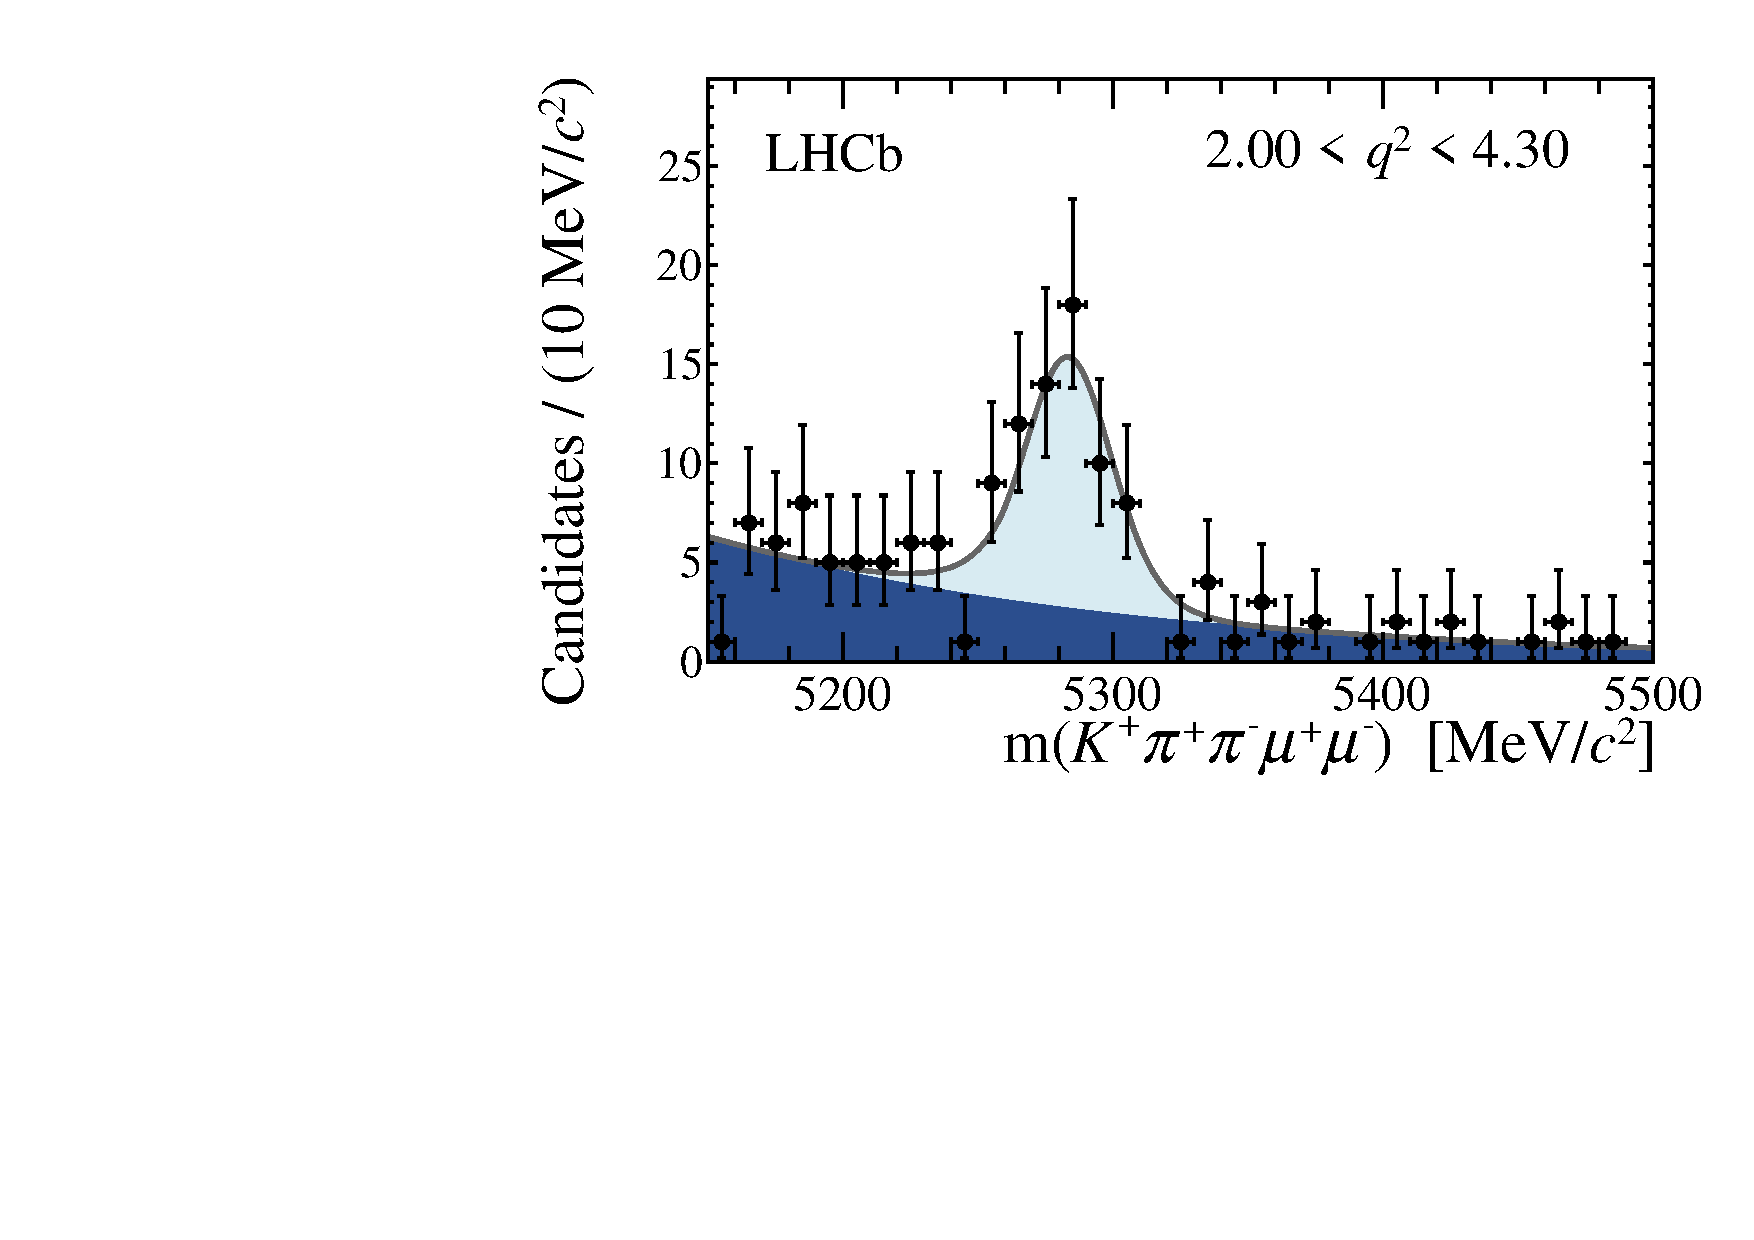
\includegraphics[width=0.48\textwidth]{kpipimumu_q2_r3}
    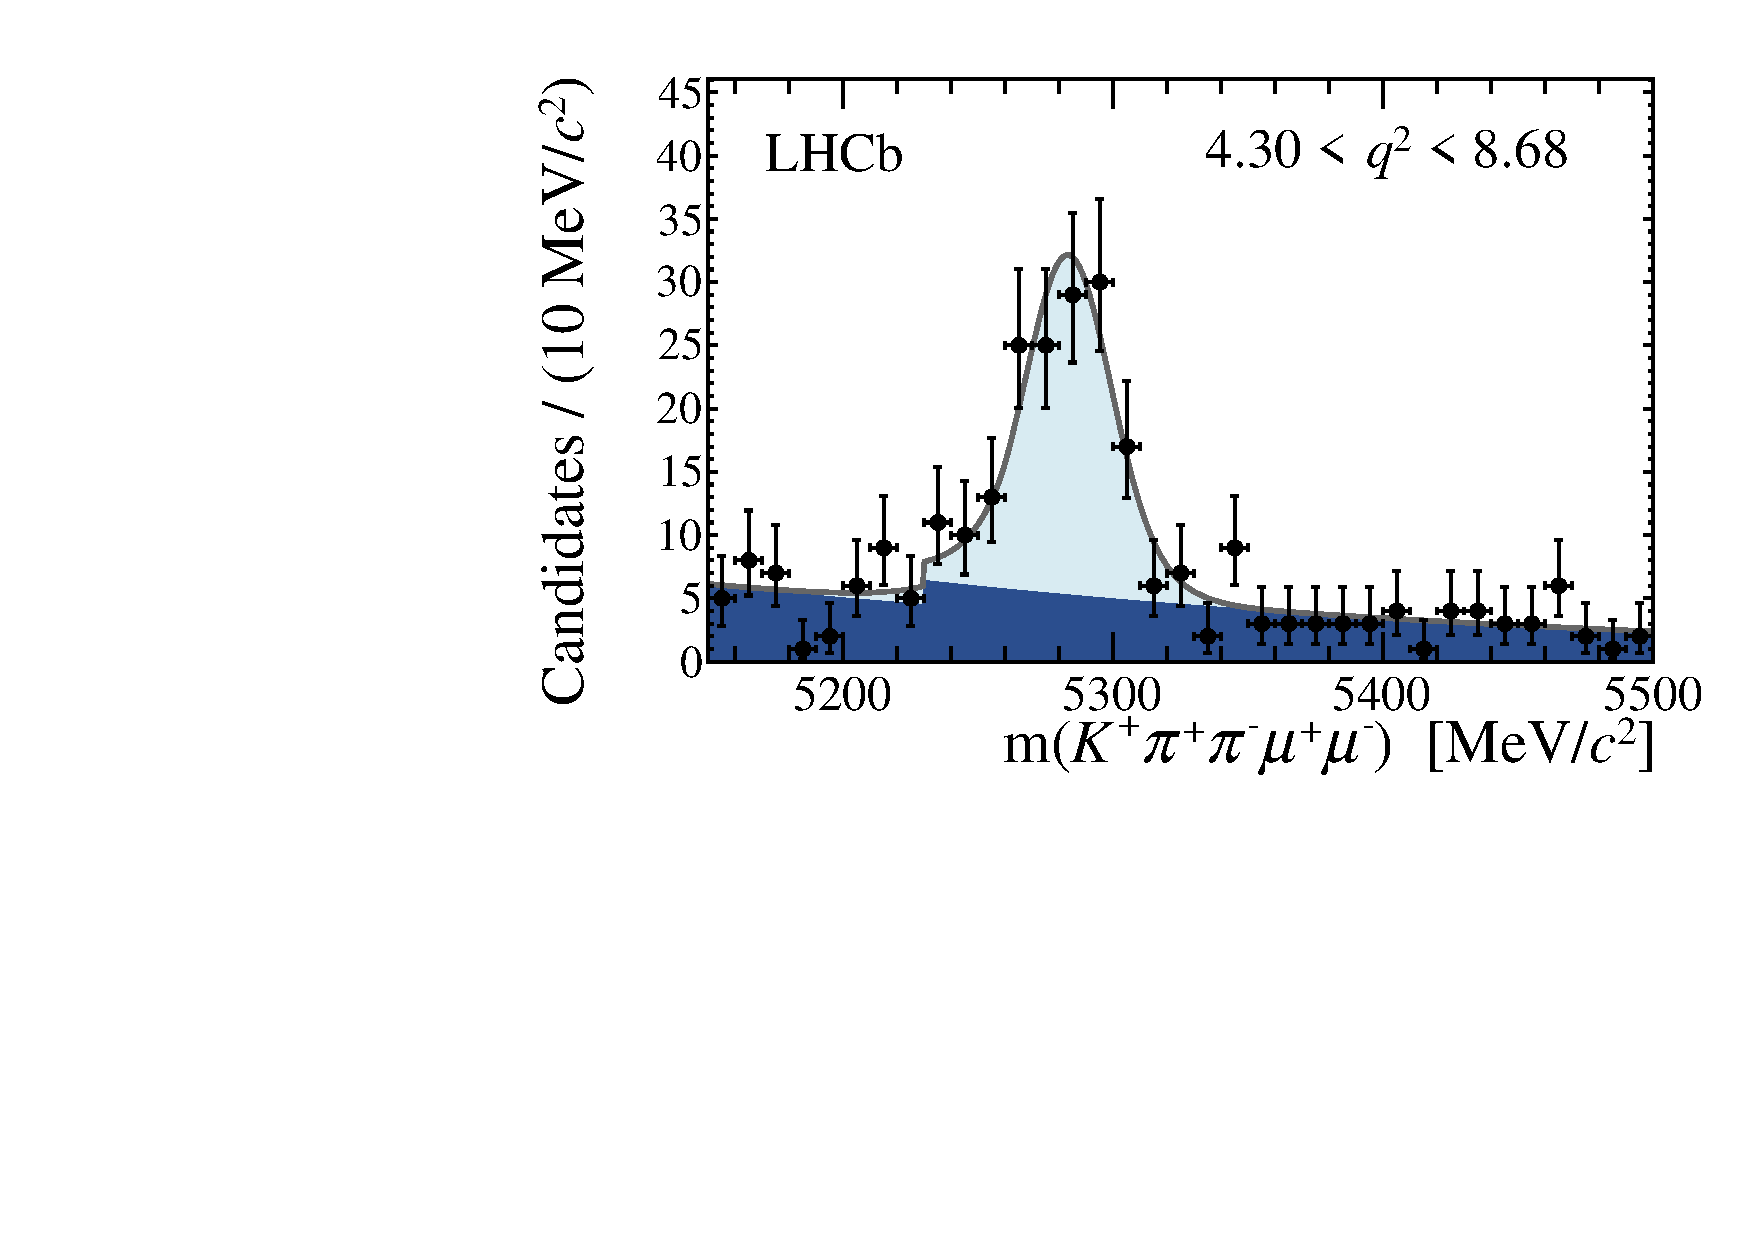
\includegraphics[width=0.48\textwidth]{kpipimumu_q2_r4}
    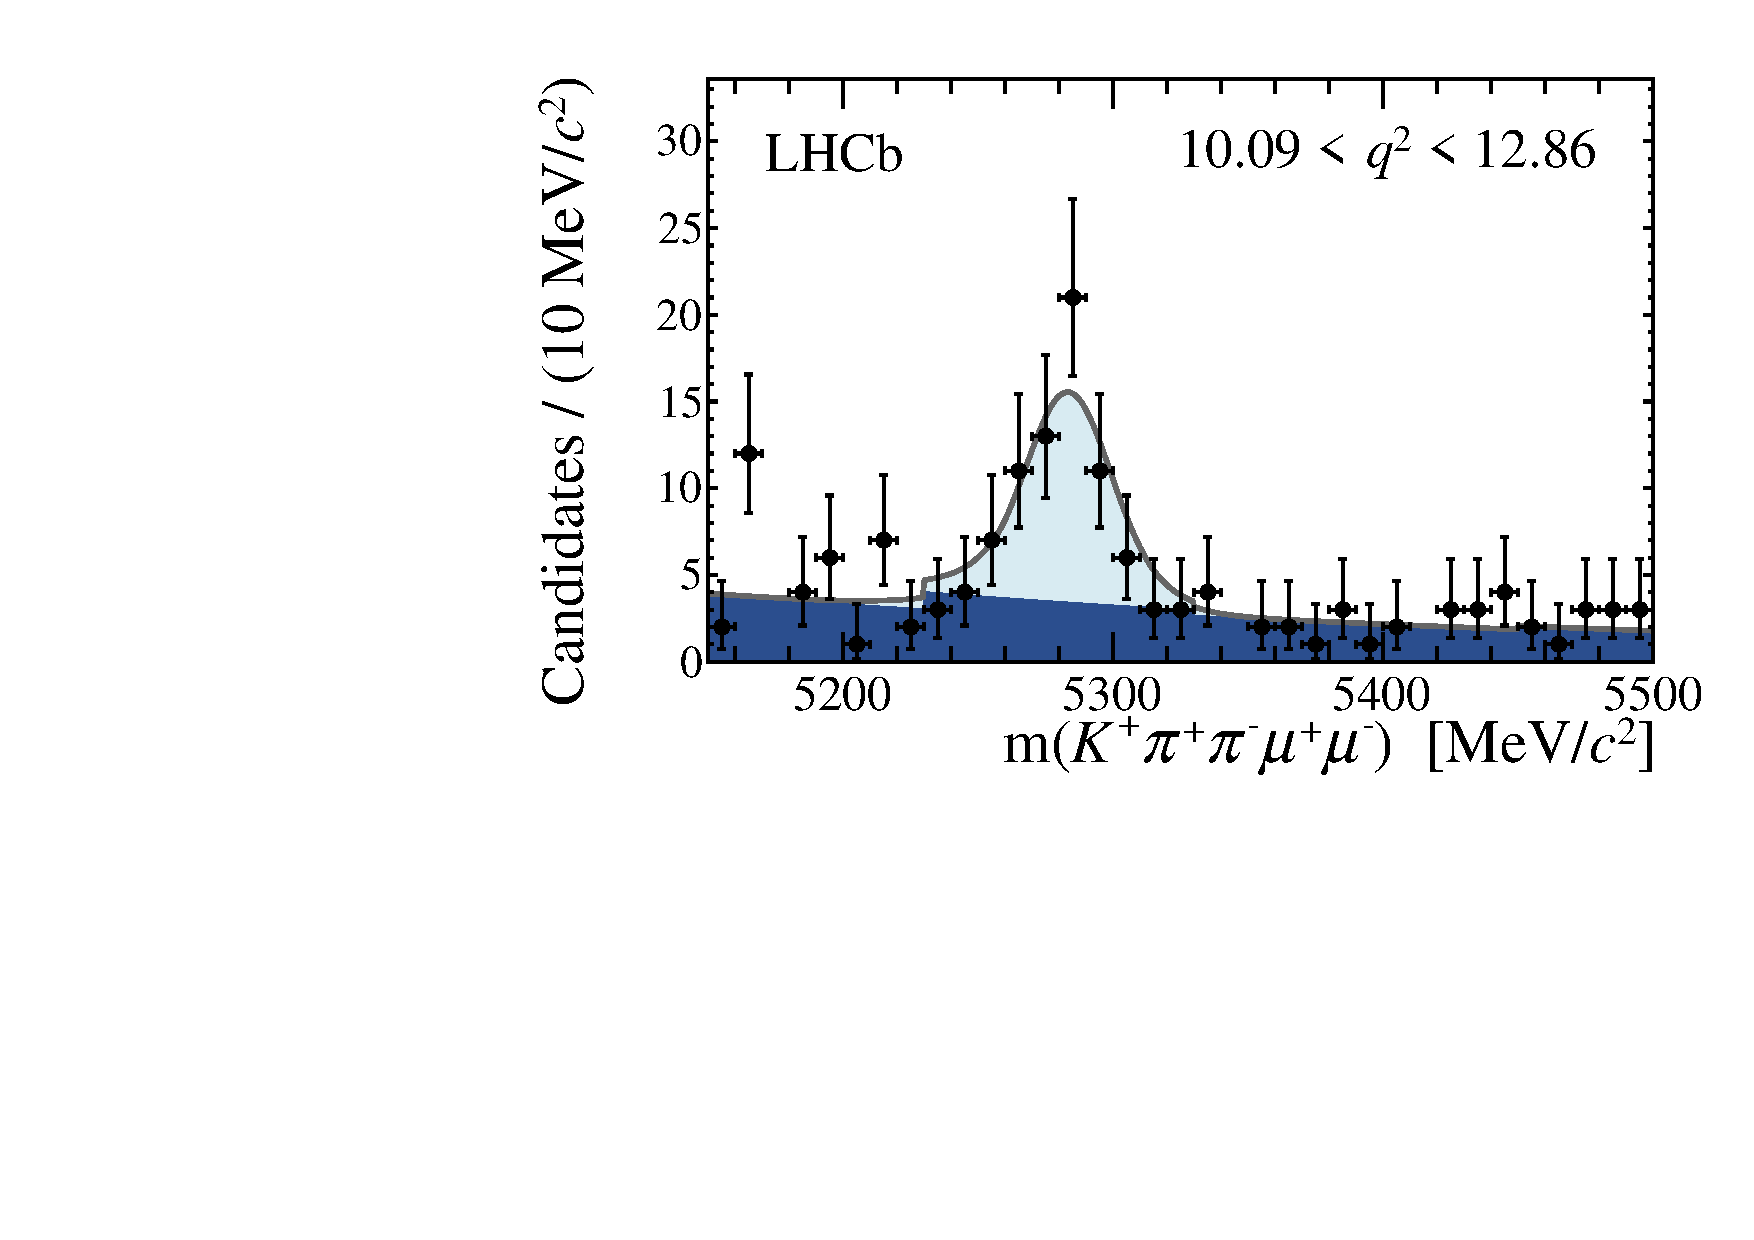
\includegraphics[width=0.48\textwidth]{kpipimumu_q2_r5}
    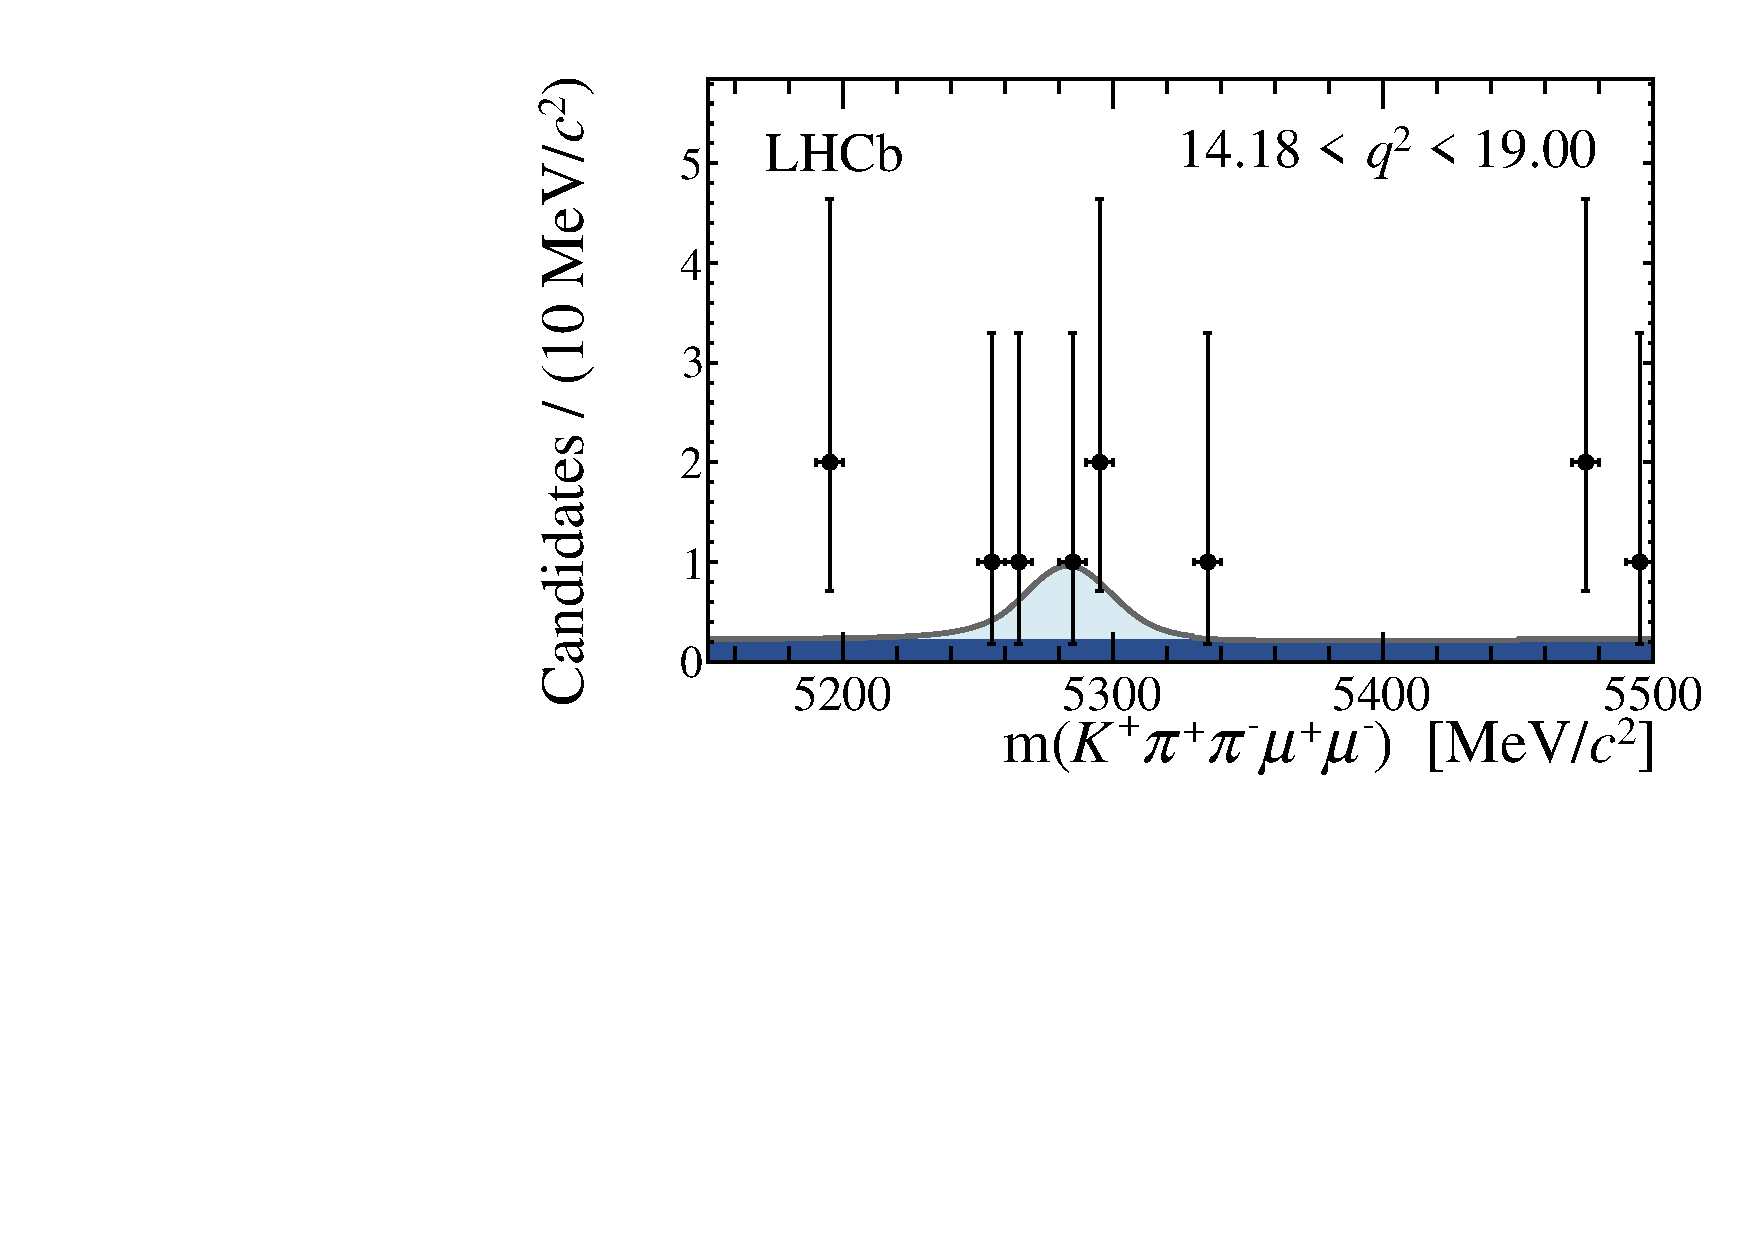
\includegraphics[width=0.48\textwidth]{kpipimumu_q2_r6}
    \caption{\small
      Invariant mass distributions of \btokpipimumu candidates in bins of \qsq with projections of
      fits overlaid, the upper left plot is a separate fit to the full \qsq range.
      The signal signal component (light blue) is modelled by the sum of two Gaussian
      distributions, and the background component (dark blue) is an exponential function.
      In the three \qsq bins $4.30<\qsq<8.68\gevgev$, $10.09<\qsq<12.86\gevgev$, and
      $14.18<\qsq<19.00\gevgev$ scaling factors in the background components are used to account
      the removal of the radiative tails of charmonium vetoes.
      The lower right
    }
    \label{fig:kpipi:q2fits}
  \end{center}
\end{figure}

Differential branching fractions were calculated with \Eq{eq:kpipi:diffbf} where yields were
extracted from fits in \Fig{fig:kpipi:q2fits}.
These results are shown graphically in \Fig{fig:kpipi:diffbf} and are given numerically --- along
with signal yields --- are shown in \Tab{tab:kpipi:diffbf}.
The integrated branching fraction is then calculated to be:
\begin{equation}
  \BF\big( \btokpipimumu \big)=
  \big(4.36\,^{+0.29}_{-0.27}\stat\pm0.21\syst\pm0.18\norm\big)\e{-7}.
\end{equation}
Since the uncertainty due to the normalization channel branching fraction is singnificant, the
ratio of branching fractions is also quoted
\begin{equation}
  \frac{ \BF\big( \btokpipimumu \big) }{ \BF\big( \btopsitwosk \big) } =
  \big(6.95\,^{+0.46}_{-0.43}\stat\pm0.34\syst\big)\e{-4}.
\end{equation}

{\renewcommand{\arraystretch}{1.2}
\begin{table}
  \begin{center}
    \caption{\small
      Signal yields and resulting differential branching fractions for the decay \btokpipimumu in
      bins of \qsq.
    }
    \label{tab:kpipi:diffbf}
    \begin{tabular}{ccc}\toprule
      \qsq bin $\left[\gevgevcccc\right]$
      & $N_\sig$
      & $\tfrac{\dBF}{\dqsq}\;\left[\e{-8}\pergevgevcccc\right]$
      \\\midrule
      $[\pz0.10,\pz2.00]$ & $134.1\,^{+12.9}_{-12.3}$     & $7.01\,^{+0.69}_{-0.65} \pm 0.47$ \\
      $[\pz2.00,\pz4.30]$ & $\pz56.5\,^{+\pz9.7}_{-\pz9.1}$ & $2.34\,^{+0.41}_{-0.38} \pm 0.15$ \\
      $[\pz4.30,\pz8.68]$ & $119.9\,^{+14.6}_{-13.7}$     & $2.30\,^{+0.28}_{-0.26} \pm 0.20$ \\
      $[10.09,12.86]$     & $\pz54.0\,^{+10.1}_{-\pz9.4}$   & $1.83\,^{+0.34}_{-0.32} \pm 0.17$ \\
      $[14.18,19.00]$     & $\pzz3.3\,^{+\pz2.8}_{-\pz2.1}$ & $0.10\,^{+0.08}_{-0.06} \pm 0.01$ \\
      %\midrule
      %$[\pz1.00,\pz6.00]$ & $144.8\,^{+14.9}_{-14.3}$     & $2.75\,^{+0.29}_{-0.28} \pm 0.16$ \\
      \bottomrule
    \end{tabular}
  \end{center}
\end{table}
}

\begin{figure}
  \begin{center}
    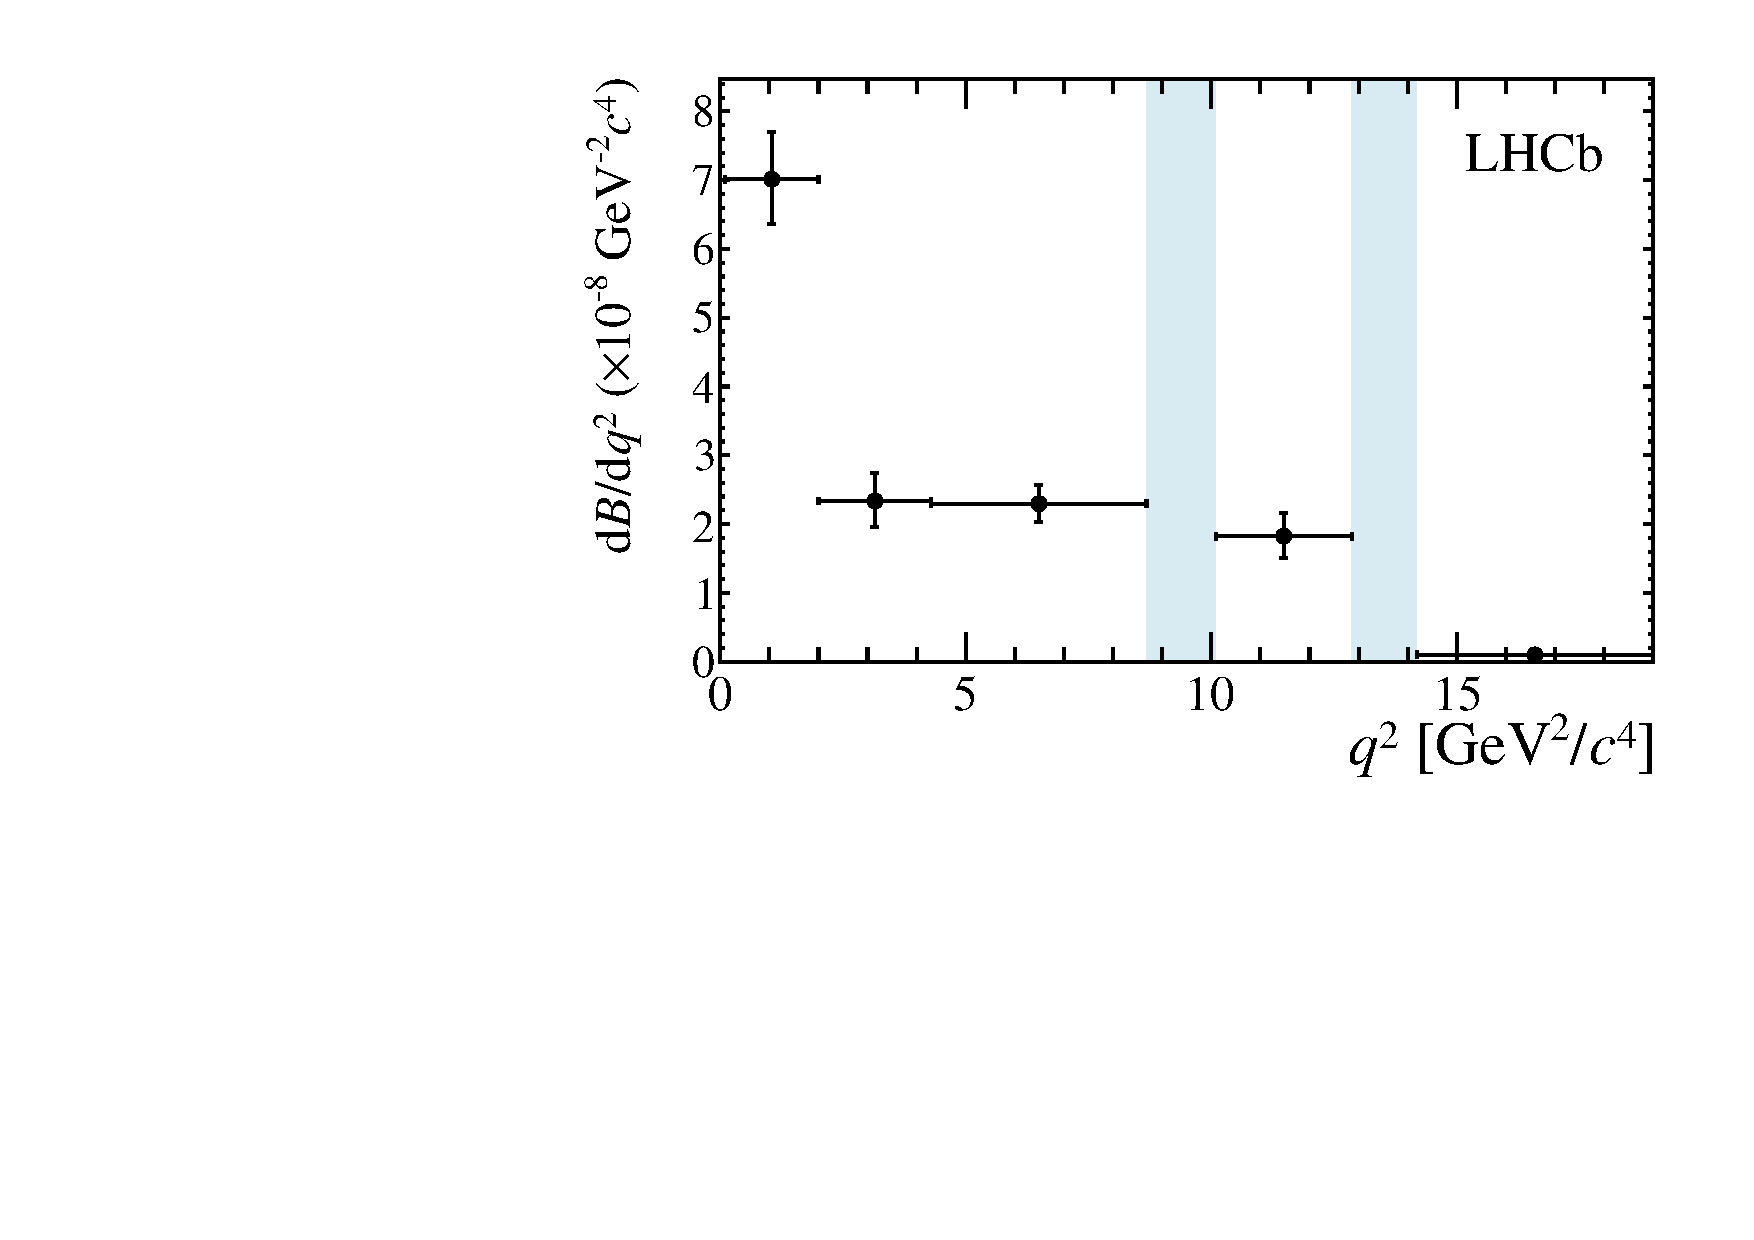
\includegraphics[width=0.48\textwidth]{diffbf}
    \caption{\small
      Differential branching fraction $\tfrac{d}{\dqsq}\BF\left(\btokpipimumu\right)$
      (as given in Table~\protect\ref{tab:hhh:diffbf}), where the
      errors shown include both statistical and systematic uncertainties.
      Shaded areas indicate the vetoed \jpsi and \psitwos resonances.
    }
    \label{fig:kpipi:diffbf}
  \end{center}
\end{figure}

Figure~\ref{fig:kpipi:kpipi} subtracted invariant mass distrributions of the \kpipi systems in the
cases for both decays \btojpsikpipi and \btokpipimumu.
Numerous broad resonances are visible in the distributions.
The \kpipi system from the resonant \btojpsikpipi decay shows significant, though not dominant,
contributions from the \kone{1270} state.
There is also a contribution visible as $m_\kpipi\simeq1750\mev$, similar to resonances seen by
\belle~\bam{ref}.



%The fits to the mass distributions to the decays \btojpsikpipi and \btokpipimumu
%sWeighted~\cite{splot} invariant mass distributions of the \kpipi systems.
%The in
%
%Due to the high statistics of the decay \btokpipimumu, its braching fraction was also measured
%differentially, in bins of the invariant mass squared of the dimuon system (\qsq).
%
%Measurements pertaining to the decay \btokpipimumu were made with respect to the normalization
%channel \btopsitwosk, where \psitwostojpsipipi and \jpsitomumu.
%\begin{equation}
  %\BF\left(\b\right)
%\end{equation}
%The decay \btojpsikpipi was used for cross-checks
%These measurements were made with respect to the normalization channels

\begin{figure}
  \begin{center}
    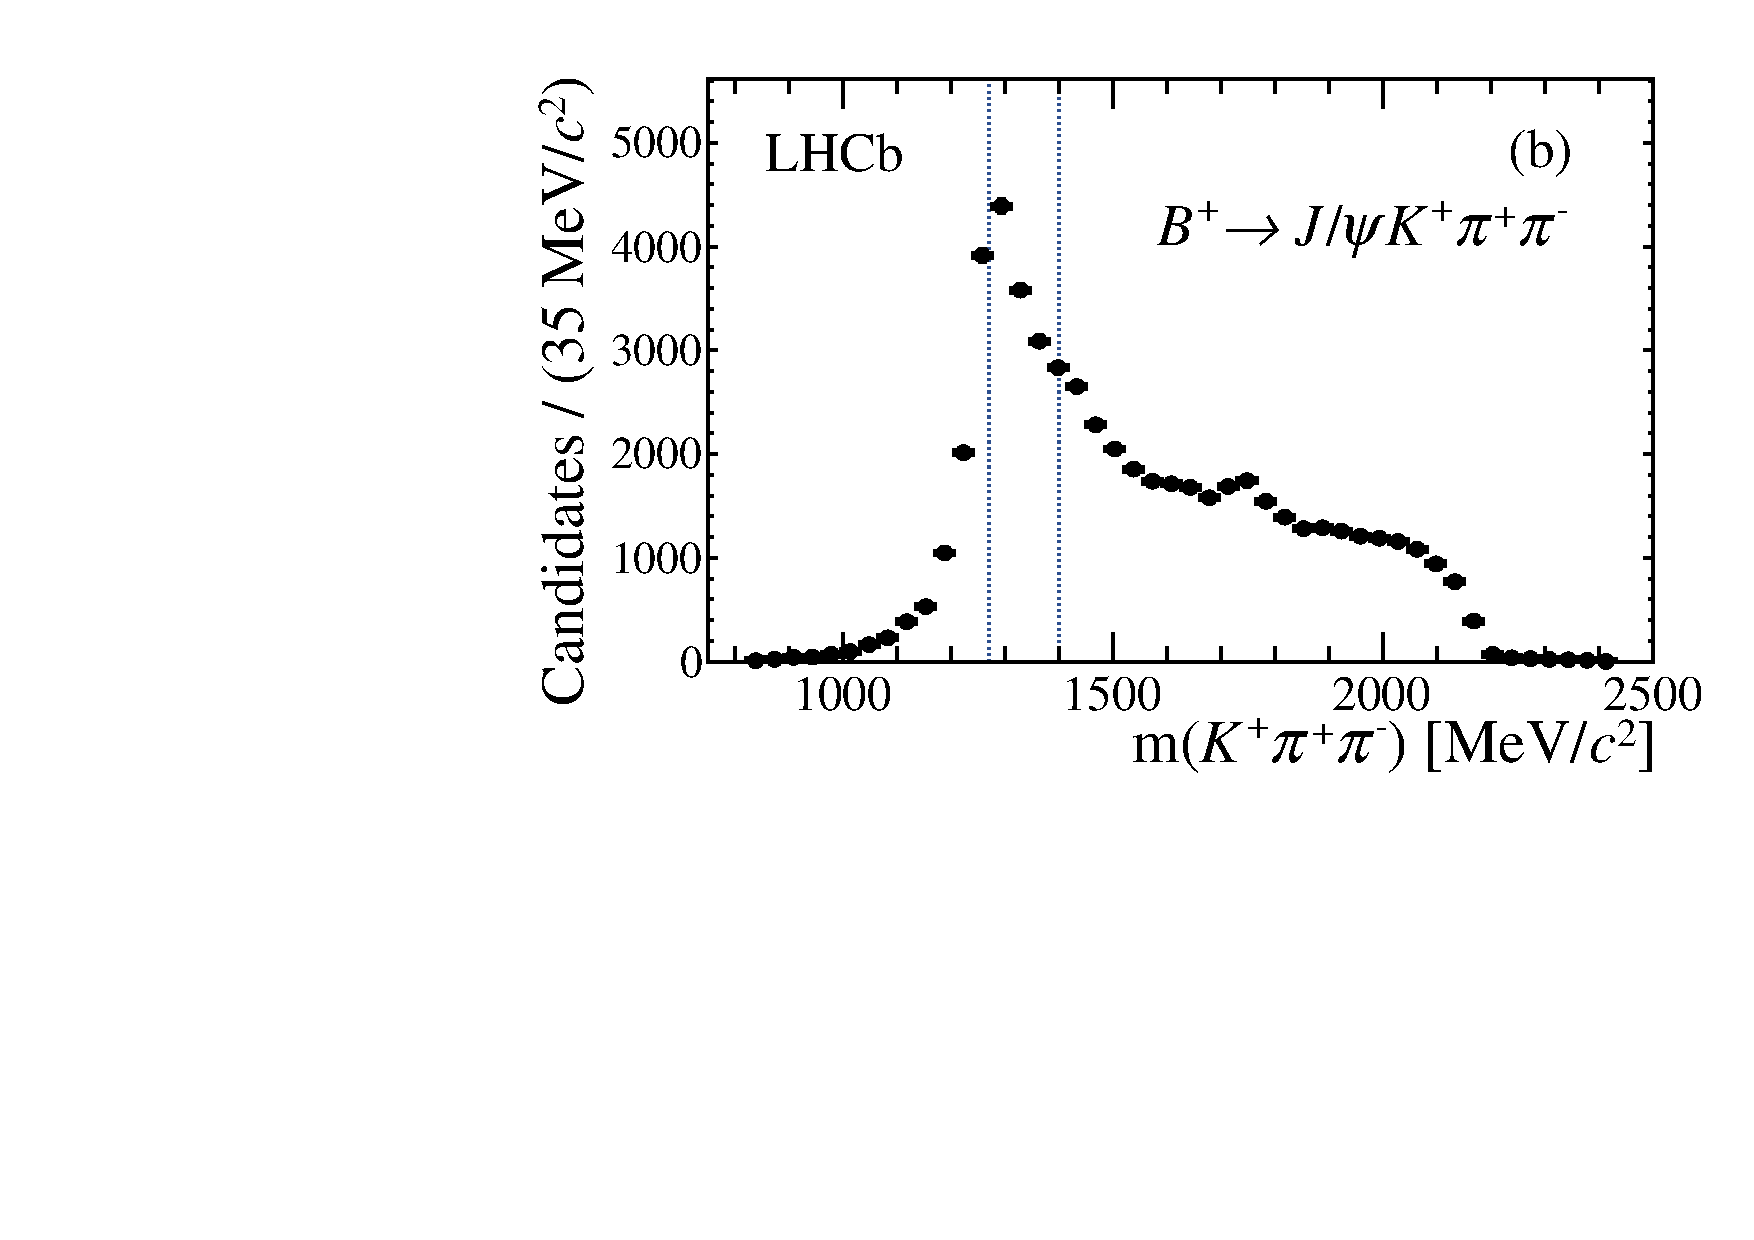
\includegraphics[width=0.48\textwidth]{kpipi_fromjpsi}
    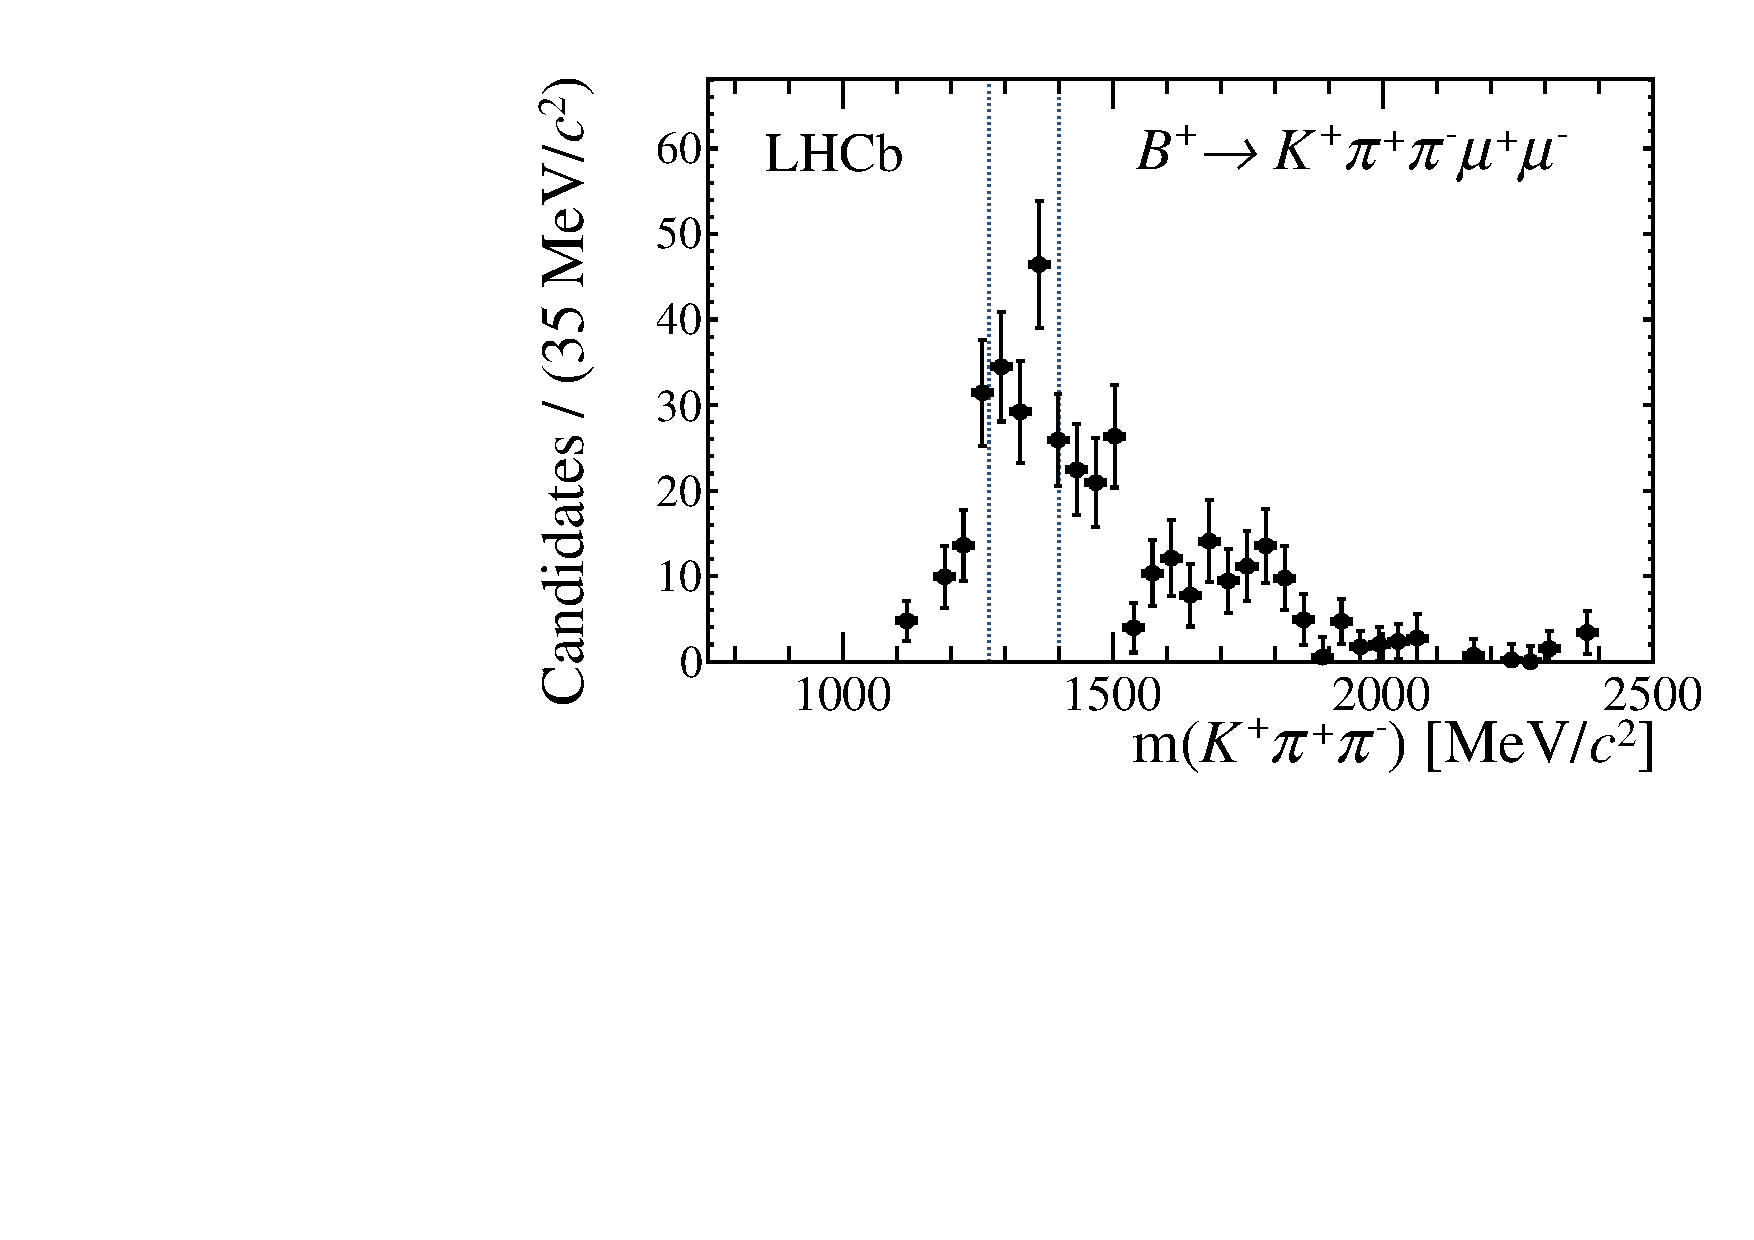
\includegraphics[width=0.48\textwidth]{kpipi_frommumu}
    \caption{\small
      Invariant mass distributions of the \kpipi object, from the
      (a) signal decay \btokpipimumu and the
      (b) control channel \btojpsikpipi which have been background subtracted
      using the \emph{sPlot}~\cite{splot} technique.
      The vertical lines indicate the central masses of the \kone{1270} and \kone{1400}
      resonances.
    }
    \label{fig:kpipi:kpipi}
  \end{center}
\end{figure}



\subsection{Systematic uncertainties}





















